\documentclass[12pt]{article}

\usepackage[dvips,letterpaper,margin=0.75in,bottom=0.75in]{geometry}
\usepackage{cite}
\usepackage{slashed}
\usepackage{graphicx}
\usepackage{amsmath}
\usepackage{braket}
\usepackage{latexsym,amssymb,amsmath}
\usepackage{pdfpages}
\usepackage{xcolor}

%
% Make ECS 32/36 options explicit
% Think about relaxing 104B requirement for A part.  112?
% Figure with prerequisite structure
%

\usepackage[american,fulldiode]{circuitikz}
\tikzset{component/.style={draw,thick,circle,fill=white,minimum size =0.75cm,inner sep=0pt}}

\begin{document}
\ctikzset{bipoles/thickness=1}
\ctikzset{bipoles/length=.6cm}

\title{Straw Man Proposal for the \\ Undergraduate Physics Curriculum}
\author{Michael Mulhearn}

\maketitle

\section{Objectives}

\begin{table}
\caption{Typical schedule for undergraduate physics majors, taking the 9H series, in the fall quarter, omitting lab courses.}
\label{tbl:current-honors}
\begin{center}
\begin{tabular}{|l|l|l|l|}
\hline
year      & fall    & winter & spring  \\
\hline
Freshman  & 9HA  & 9HB  & 9HC \\
\hline
Sophomore & 9HD  & 9HE   & 40     \\
          &      &        &        \\
\hline
Junior    & 104A & 105B & 110B\\
          & 105A & 110A & 115A\\
\hline
Senior    & 115B &        & \\
          & 110C &        & \\
          & 112  &        & \\

\hline 
\end{tabular}
\end{center}
\end{table}

\begin{table}
\caption{Typical schedule for undergraduate physics majors that transfer to UC Davis in their Junior year, omitting lab courses.}
\label{tbl:current-transfers}
\begin{center}
\begin{tabular}{|l|l|l|l|}
\hline
year      & fall    & winter & spring  \\
\hline
Junior    & 9D  &    & 40     \\
          & 104A & 105B & 110B\\
          & 105A & 110A & 115A\\
          & 102 &       & \\
\hline
Senior    & 115B &        & \\
          & 112  &        & \\
\hline 
\end{tabular}
\end{center}
\end{table}

The current typical schedule of student coursework is shown in Table~\ref{tbl:current-honors} for honors students.  The schedule for transfer students that arrive at UC Davis for their Junior year is shown in Table~\ref{tbl:current-transfers}.  There are of course many students taking different trajectories through our program, but most are some variation on these two.  This proposal aims to improve upon this course of study, to achieve the following aims:
\begin{itemize}

\item Physics majors that complete 9HD or 9D in the fall of their sophomore year have little to do for the rest of the year.  The honors students have 9HE, but this is effectively an elective and does little to further prepare them for upper division course work.  The recent addition of 40 and 80 helps somewhat, but not enough.  The result of this stalling is that the junior and senior year are a race to complete the degree requirements, leaving very little flexibility or time for advanced electives.

\item Transfer students that arrive at UC Davis for their Junior year face a wall of coursework that they have to handle in the first quarter: math methods, mechanics, and modern physics.  Many also take Physics 102, which is nominally a one credit course, but generally nearly as much work as a four credit course.  For many of the transfer students these courses are the first physics courses that require solving challenging homework problems, and they face effectively 16 credits.  We have two trains of students running through our program (transfers and honors students) and the fall of their junior year is the train wreck where they collide.

\item The current curriculum does not include sufficient computing practice for our students.  It's useful to consider what a physics degree would like if we taught calculus the same way we teach computing.  Students would arrive their Freshman year and take an introductory calculus course.  Then, they would take their physics courses, which would never mention calculus.  At some point in their Junior or Senior year, they would take a one quarter course called "Calculus in Physics" that would attempt to show all the ways we use calculus in physics.  Our students are experts at calculus because they learn how to use the tool, and then apply it, again and again, throughout their coursework.  To remain relevant in the modern world (or even the world from 20 years ago, to be honest) our majors need more practice in the use of computing as a tool for solving physics problems.

\item We are allowed to require a maximum of 110 credits from the college of Letters and Science, which is one half the maximum number of credits students are allowed to take.  Fitting the canon of undergraduate physics into such a tight space is extremely challenging.  Students complain that we waste time teaching some topics again and again (e.g. Special Relativity from scratch) while completely dropping other topics (e.g. Classical Hamiltonians).  The problem is particularly acute for Applied Physics majors, where core material must be dropped to make space for coursework outside of Physics.

\item The prerequisite structure of the upper division courses creates many tiers.  
As an extreme example, 122 requires 112, which requires 115A, which requires 104A and 105A, both of which require the 9 series.  This, combined with the rapid paces, leaves very little flexibility for students once they start their Junior year.  For example, missing a single quarter of the courses in the Junior year of Table~\ref{tbl:current-honors} requires an exception to prerequisites or an extra year to graduate.

\label{tbl:current-honors}

\end{itemize}

A proposal to improve on all of these issues is detailed in the next section followed by a discussion of non-lab coursework, computational lab work, and experimental lab work in turn, and pre-requisite structure.
\newpage

\section{B.S. Requirements (Minimal)}

The proposed B.S. Requirements are presented in Tables~\ref{tbl:prep} and \ref{tbl:core}.  Example schedules are presented in Tables~\ref{tbl:proposed-honors} and \ref{tbl:proposed-transfers}.

\begin{table}
\caption{\label{tbl:prep}Preparatory Subject Matter}
\noindent
\vskip 0.25cm
Credits:  49-50. *: recommended, C: concurrently.\\
\begin{tabular}{|llllll|}
\hline
Course & & Credits & Offered & Pre-reqs & Name \\
\hline
PHY & 9A & 5 & F,S & & Classical Physics {\it (Class. Mech.)}\\ 
    & 9B & 5 & F,W & & Classical Physics {\it (Waves, Thermo., Optics.)}\\ 
    & 9C & 5 & W,S & & Classical Physics {\it (Elec. and Magn.)}\\ 
    & 9D & 4 & F,S & & Modern Physics {\it (Rel. and Quant. Mech.)}\\ 
\hline
&or&&\\
\hline
PHY & 9HA & 5 & F & & Honors Physics {\it (Class. Mech.)}\\ 
    & 9HB & 5 & W & & Honors Physics {\it (Rel. and Stat. Mech.)}\\ 
    & 9HC & 5 & S & & Honors Physics {\it (Waves and Quant. Mech.)}\\ 
    & 9HD & 5 & F & & Honors Physics {\it (Elec. and Magn.)}\\ 
\hline
\hline
MAT & 21A & 4 & & &\\ 
    & 21B & 4 & & &\\ 
    & 21C & 4 & & &\\ 
    & 21D & 4 & & &\\ 
    & 22A & 3 & & &\\ 
    & 22B & 3 & & &\\ 
PHY & 40  & 4 & S & & Introduction to Physics Computation \\ 
    & 80  & 4 & (F),W,S & 40,9D & Experimental Techniques \\ 
PHY & 185* & 1 & S & & \\ 
    & 190* & 1 & F & & \\ 
\hline
\end{tabular}
\end{table}

\begin{table}
\caption{\label{tbl:core}Core Subject Matter}
\noindent
\vskip 0.25cm
Credits:  46-50. *: recommended, C: concurrently.\\
\begin{tabular}{|llllll|}
\hline
Course & & Credits & Offered & Pre-reqs & Name \\
\hline
PHY & 102  & 4 & W & 40, 9D     & Computational Physics\\
    & 104A & 4 & F & C:9D       & Mathematical Physics \\ 
    & 105A & 4 & W & 104A, 9D   & Classical Mechanics I\\
    & 105B & 4 & S & 105A, 102  & Classical Mechanics II\\ 
    & 110A & 4 & W & 104A, 9D   & Electricity and Magnetism I\\
    & 110B & 4 & S & 110A, 102  & Electricity and Magnetism II\\
    & 115A & 4 & F & 104A, 9D   & Quantum Mechanics I \\
    & 115B & 4 & W & 115A, 102  & Quantum Mechanics II \\
    & 115C & 4 & S & 115B       & Applications of Quantum Mechanics\\ 
    & 112  & 4 & F & 104A, 9D   & Thermodynamics and Statistical Mechanics\\    
\hline
PHY & 116A & 4 &  W & 80   & Instrumentation with Discrete Electronics  \\
    & 116B & 4 &  S & 116B & Instrumentation with Integrated Electronics\\ 
\hline
    & or & & & & \\
\hline
PHY & 122A or B & 4 & (F),W,S & & Advanced Physics Laboratory \\  
\hline
 & Any two of & & & & (all three recommended): \\
\hline 
PHY & 105L & 1 & S & 102,C:105B & Computational Lab in Mechanics \\
    & 112L & 1 & F & 102,C:112  & Computational Lab in Statistical Mechanics \\ 
    & 115L & 1 & W & 102,C:115B & Computational Lab in Quantum Mechanics \\ 
\hline
\end{tabular}\\ \vskip 0.25cm
\noindent
{\bf Electives:} an additional 15 credits of electives is required, 12 credits from advanced (capstone) topics.\\
\noindent
{\bf Total Units:} 110-115
\end{table}

\begin{table}
\caption{Example schedule for undergraduate physics majors taking the 9H series and opting for the 116 lab sequence.  E is an elective course.  Rate is 5-9 credits per quarter.}
\label{tbl:proposed-honors}
\begin{center}
\begin{tabular}{|l|l|l|l|}
\hline
year      & fall    & winter & spring \\
\hline
Freshman  & 9HA(5)  & 9HB(5)  & 9HC(5) \\
          &         &         & 40(4)  \\
\hline
Sophomore & 9HD(5)  & 105A(4) &  105B(4) \\
          & 104A(4) & 102(4)  &  105L(1) \\
          &         &         &  80(4)\\
\hline
Junior    & 115A(4) & 115B(4)  & 115C(4)\\
          & 112(4)  & 110A(4)  & 110B(4)\\
		  & 112L(1) & 115L(1)  & \\
\hline
Senior    & E(4)    & 116A(4)  & 116B(4) \\
          & E(4)    & E(4)     & E(4) \\

\hline  
\end{tabular}
\end{center}
\end{table}

\begin{table}

\caption{Example schedule for for an undergraduate physics majors that transfered to UC Davis in their Junior year without Physics D or 40 equivalents.  Rate is 12-13 credits per quarter.}
\label{tbl:proposed-transfers}
\begin{center}
\begin{tabular}{|l|l|l|l|}
\hline
year      & fall    & winter & spring \\
\hline
Junior   & 9D(4)     & 105A(4)       & 105B(4) \\
         & 40(4)     & 110A(4)       & 105L(1) \\         
         & 104A(4)   & 102(4)        & 110B(4) \\
         &           &               & 80(4) \\
\hline
Senior   & 115A(4)   & 115B(4)       & 115C(4) \\
         & 112(4)    & 122A(4)       & E(4) \\
         & 112L(1)   & E(4)          & E(4)  \\
		 & E(4)      & 115L(1)       & \\
\hline 
\end{tabular}
\end{center}
\end{table}

\newpage
\section{Discussion of Regular Coursework}

The typical schedule of courses for the proposed new curriculum is shown in Table~\ref{tbl:proposed-honors} for honors physics and Table~\ref{tbl:proposed-transfers} for Junior transfer students.
The primary feature is that incoming transfer students now overlap mostly with sophomore honors physics students.  This eliminates the stalling of our honors students while relieving some of the intense academic pressure on incoming transfer students.  Our experience has been that the best of the transfer students perform as well as our four-year students once they have sufficient time to adjust, and this proposal gives them that time.  Accelerating the honors students also provides tremendous additional flexibility to their schedule.  Transfer students that wish to complete their degree in two-years are still highly constrained, but instead of facing a 13 credit brick wall, they start with only eight credits of required coursework in their first fall quarter at UCD.

Several new classes have been added and others require changes to their content or will no longer be required:
\begin{itemize}
\item 9A-D and 9HA-D  These courses are largely unchanged, however, some fine adjustments may be needed to ensure that the 9 series plus 104A are sufficient preparation for 115A and 112.
\item 9HE is no longer offered:  This course is effectively an elective, with content that varies from instructor to instructor.  By removing it, we allow the Honors students to start toward the core material sooner, leaving more time for advanced electives. With more relaxed schedule in their senior year, it seems highly plausible that physics majors will take more electives.
\item The 115 sequence will be substantially revised.  The addition of 115C as a third quarter is intended to achieve a number of effects to the entire sequence.  115A will be an introduction to QM that relies only on 9 series and 104B, and it should function well as a standalone course for applied physics majors who will not be required to take 115B and 115C.  The next two quarters, 115B and 115C, have 102 as prerequisites and can therefore integrate significant computational work into the curriculum.  The extra time should also allow coverage of new topics (e.g. QIT).
\item 102:  This course will be renamed ``Computational Physics'' and will be closer in content to the 104B as taught by some instructors.  This course will play a more integral role in this revised curriculum and so the content and tools will need to be more consistently covered than in 104B.  The decision to use 102 as the course number is for clarity, as 104A will not be a prerequisite.
\item 110C is no longer offered:  A third quarter of E+M is too much to allocate to this topic, given the other needs of the curriculum and limited number of required credits. 110A and B will need some adjustment to make certain that the vector potential and special relativity are covered.
\end{itemize}

\section{Discussion of Computational Physics}
One of the major objectives of this curriculum overhaul is to better integrate computational physics throughout the curriculum, and this is accomplished in a number of ways:
\begin{itemize}
\item The one credit PHY 102 course is eliminated.  Now every major takes PHY 40 and a new 4 credit PHY 102 for a total of eight credits of introductory programming and computational physics. 
\item Physics 80 is required for all majors and includes extensive use of scientific python for data analysis and presentation.
\item There are three new one-credit computational lab courses (105L, 112L, and 115L) designed to be taken concurrently with 105B, 112, and 115B. They are computational problem solving labs related to mechanics, E+M, and quantum mechanics.  The instructor will present a technique and problem during a single one hour lecture, and the students will have the rest of the week to complete their assignment.  It is expected that one instructor will teach all three in a single year, which will count as one course.
These are each offered in a different quarters, so students get three credits of computational problem-solving spread across an entire year.  Due to credit limits, we only require two of these courses, but all three are recommended.
\item PHY 105B, 110B, and 115B now have 102 (computational physics) as a pre-requisite.  Computational problems can therefore be fully integrated into these courses.
\end{itemize}

\section{Discussion of Labs}

Physics 80 was introduced in 2018, and is currently a pre-req for 122A and 122B.  It is anticipated that this will relieve some of the time pressure in this one quarter course.

In this proposal, Physics 80 is a pre-requisite for the 116 (Instrumentation) sequence.  Physics 80 covers some of the content in 116A (passive analog electronics) and some of the content in 116C (computation with scientific python and statistical analysis).  Therefore, the three quarter 116 sequence (A,B, and C) can become a two quarter sequence, 116A covers discrete electronics (analog and digital), and 116B can cover integrated electronics (microprocessors and FPGAs).

\section{Discussion of Prerequisites}

\begin{figure}
\begin{center}
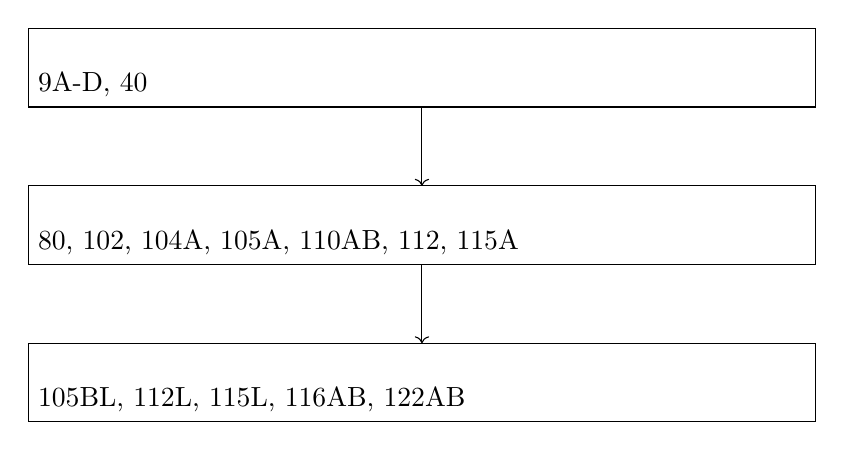
\begin{tikzpicture}
\draw (0,0) -- ++(0,1) -- ++(10,0) -- ++(0,-1) -- ++(-10,0);
\node[above right] at (0,0) {9A-D, 40};
\draw (0,-2) -- ++(0,1) -- ++(10,0) -- ++(0,-1) -- ++(-10,0);
\node[above right] at (0,-2) {80, 102, 104A, 105A, 110AB, 112, 115A};
\draw (0,-4) -- ++(0,1) -- ++(10,0) -- ++(0,-1) -- ++(-10,0);
\node[above right] at (0,-4) {105BL, 112L, 115L, 116AB, 122AB};
\draw[->] (5,0) --(5,-1);
\draw[->] (5,-2) --(5,-3);
\end{tikzpicture}
\caption{\label{fig:prereqs} The prerequisite structure of required courses.  At each tier, course prerequisites can only be earlier courses in the same sequence or courses from a previous tier.  Courses from the lowest tier should not be prerequisites for any other courses outside their own sequence, including capstone courses.}
\end{center}
\end{figure}

An overview of the prerequisite structure is shown in Fig.~\ref{fig:prereqs}.  Classes within a tier can require only earlier classes from within the sequence (e.g. B requires A) or classes from an earlier tier.  One exception is that 104A requires 9D (which may be taken concurrently).  Reducing the number of tiers in our program to three affords significantly more flexibility for students to work through each tier in whatever order works best for their schedule.  Because 102 requires 40 and the 9 series, but is needed for 115B and 105B, it remains a potential bottleneck, along with 104B.  The limited number of offerings for most courses will also limit flexibility in practice.

The most notable changes are that:
\begin{itemize}
\item 115A does not require 105A anymore, 9A-D must suffice instead
\item 112 does not require 115A anymore, 104A and 9A-D must suffice instead
\item The new four-credit 102 course (which replaces both 104B and the current version of 102) does not require 104A, and instead requires 40.
\item 105B and 115B require 102, which allows for computing to be integrated with the course. 
\end{itemize}
Some classes can be globally substituted as prerequisites, which we note here:
\begin{itemize}
\item 9HD can replace 9D or 9C.  Note that 9HC does not replace 9C due to different ordering of the Honors sequence.
\item Any ECS introductory programming course can replace 40.
\end{itemize}

\section{Other Goals}
There are some other goals not included in this proposal that I would like to keep track of:
\begin{itemize}
\item It would be nice if e.g. 105A, 110A-B, 115A worked as complete set of core courses for e.g. Astro and Applied physics majors. 
\item I would like to offer some sort of lower division 3 credit elective for the transfer students (PHY 19?) to take in Fall of their Junior year, that focuses on solving problems from material in 9A-C.  We could also recommend this to students that didn't did so well in 9 and can use a bit of brushing up before the upper division course work.  Currently, 105A is filling this role.
\end{itemize}

\end{document}

\section{Detailed course listings - Preparatory Material}

For reference, the content in core required courses in the present catalog is included here:

\begin{itemize}

\item {\bf PHY 9A - Classical Physics (5)}
{\it Lecture—3 hours; laboratory—2.5 hours; discussion—1 hour. Prerequisite: Mathematics 21B. Introduction to general principles and analytical methods used in physics for physical science and engineering majors. Classical mechanics. Only 2 units of credit to students who have completed course 1A or 7B. Not open for credit to students who have completed course 9HA. GE credit: SciEng | SE. - III. (III.)}

\item {\bf PHY 9B - Classical Physics (5)}
{\it Lecture - 3 hours; laboratory - 2.5 hours; discussion - 1 hour. Prerequisite: course 9A [or 9HA], Mathematics 21C, 21D (may be taken concurrently). Continuation of course 9A. Fluid mechanics, thermodynamics, wave phenomena, optics. Only 2 units of credit to students who have completed course 7A. Not open for credit to students who have completed course 9HB, 9HC, or Engineering 105. - I. (I.)}

\item {\bf PHY 9C - Classical Physics (5)}
{\it Lecture - 3 hours; laboratory - 2.5 hours; discussion - 1 hour. Prerequisite; course 9B [or 9HC], Mathematics 21D, 22A (may be taken concurrently). Electricity and magnetism including circuits and Maxwell’s equations. Only 3 units of credit to students who have completed course 7C. Not open for credit to students who have completed course 9HD. GE credit: SciEng | SE. - II. (II.)}

\item {\bf PHY 9D - Modern Physics (4)}
{\it Lecture - 3 hours; discussion - 1.5 hours. Prerequisite: course 9C [or 9HD] and Mathematics 22A; Mathematics 22B recommended (may be taken concurrently). Introduction to physics concepts developed since 1900. Special relativity, quantum mechanics, atoms, molecules, condensed matter, nuclear and particle physics. Not open for credit to students who have completed course 9HB, 9HC, or 9HE. GE credit: SciEng | SE.- III. (III.)}

\item {\bf PHY 9HA - Honors Physics (5)}
{\it Lecture - 3 hours; discussion/laboratory - 4 hours. Prerequisite: Mathematics 21B (may be taken concurrently) or consent of instructor. Classical mechanics. Same material as course 9A in greater depth. For students in physical sciences, mathematics, and engineering. Only 2 units of credit to students who have completed course 7B. Not open for credit to students who have completed course 9A. GE credit: SciEng | SE. - I. (I.)}

\item {\bf 9HB - Honors Physics (5)}
{\it Lecture - 3 hours; discussion/laboratory - 4 hours. Prerequisite: Physics 9HA or 9A, Mathematics 21C (may be taken concurrently). Special relativity, thermal physics. Continuation of course 9HA. Only 2 units of credit to students who have completed course 7A. Not open for credit to students who have completed course 9B or 9D. GE credit: SciEng | SE. - II. (II.)}

\item {\bf 9HC - Honors Physics (5)}
{\it Lecture - 3 hours; discussion/laboratory - 4 hours. Prerequisite: course 9HB and Mathematics 21D (may be taken concurrently). Waves, sound, optics, quantum physics. Continuation of Physics 9HB. Only 2 units of credit to students who have completed course 7C. Not open for credit to students who have completed course 9B or 9D. GE credit: SciEng | SE.- III. (III.)
Recent Syllabi and More Complete Descriptions}

\item {\bf 9HD - Honors Physics (5)}
{\it Lecture - 3 hours; discussion/laboratory - 4 hours. Prerequisite: course 9HC and Mathematics 21D. Electricity and magnetism. Continuation of Physics 9HC. Not open for credit to students who have completed course 9C. GE credit: SciEng | SE. - I. (I.)}

\item {\bf 9HE - Honors Physics (5)}
{\it Lecture - 3 hours; discussion/laboratory - 4 hours. Prerequisite: course 9HD and Mathematics 22B (may be taken concurrently). Application of quantum mechanics. Not open for credit to students who have completed course 9D. GE credit: SciEng | SE. - II. (II.)}

\item {\bf PHY 40 — Introduction to Physics Computation (4)}
{\it Lecture—2 hour(s); Laboratory—4 hour(s). Introduction to programming using C++ with examples from computational physics. Introduction to modern tools used for scientific analysis, including Scientific computing with Python. GE credit: SE. Effective: 2018 Summer Session 2.}

\item {\bf PHY 80 — Experimental Techniques (4)}
{\it Lecture—2 hour(s); Laboratory—5 hour(s). Prerequisite(s): PHY 009D or PHY 009HD. Open to Physics and Applied Physics majors only. Experimental techniques. Design of circuits. Data analysis, sources of noise, statistical and systematic uncertainties. Light sources, detection, and measurement in basic optical systems. Effective: 2017 Fall Quarter.}

\end{itemize}

\section{Detailed course listings - Core Subject Matter}

\begin{itemize}
\item {\bf PHY 104A - Introductory Methods of Mathematical Physics}
{\it Lecture - 3 hours; extensive problem solving. Prerequisite: courses 9B, 9C, 9D [or 9HB, 9HC, 9HD] and Mathematics 21D, 22A, and 22B with grade C- or better or consent of instructor. Introduction to the mathematics used in upper-division physics courses, including applications of vector spaces, Fourier analysis, partial differential equations. - I. (I.)}

Recently taught by Scalettar and Luty.  Luty teaches this as a boot camp for upper division courses:  vectors, expansion in small parameters, and PDEs.  All topics which are in principle should have been seen before, but students clearly need practice with problems.

\item {\bf PHY 105A - Analytical Mechanics}
{\it Lecture - 3 hours; extensive problem solving. Prerequisite: courses 9B, 9C, 9D [or 9HB, 9HC, 9HD] and Mathematics 21D, 22A, and 22B passed with grade C– or better; or consent of department; course 104A and 105A passed with a grade C– or better or consent of department required for 105B. Principles and applications of Newtonian mechanics; introduction to Lagrange’s and Hamilton’s equations. - I-II. (I-II.)}

Recently taught by Calderon, Cebra, Svoboda, and Conway.  Covers Morin 1-5.  This course is heavy on problem solving.  Morin focuses more on challenging problems, and less on mathematical formalism (e.g. leaves out Hamiltonian)
Not all instructors reach 5 in first quarter.

\item {\bf PHY 105B - Analytical Mechanics}
{\it Lecture - 3 hours; extensive problem solving. Prerequisite: courses 9B, 9C, 9D [or 9HB, 9HC, 9HD] and Mathematics 21D, 22A, and 22B passed with grade C– or better; or consent of department; course 104A and 105A passed with a grade C– or better or consent of department required for 105B. Principles and applications of Newtonian mechanics; introduction to Lagrange’s and Hamilton’s equations. - I-II. (I-II.)}

Recently taught by Pickett, Conway.  Covers Morin 6-11.  Picket supplement chapter 5 with supplemental material for Hamiltonian.

\item {\bf PHY 110A - Electricity and Magnetism}
{\it Lecture - 3 hours; extensive problem solving. Prerequisite: courses 9B, 9C, 9D [or 9HB, 9HC, 9HD] and Mathematics 21D, 22A, and 22B passed with grade C– or better, or consent of department; prerequisite for 110B is courses 110A and 104A passed with a grade of C– or better or consent of department; prerequisite for course 110C is courses 110B and 104B passed with a grade of C– or better, or consent of department. Theory of electrostatics, electromagnetism, Maxwell’s equations, electromagnetic waves. - II-III-I. (II-III-I.)}

Recently taught by Da Silva Neto and Yu.  Covers Griffiths 1-4.  Yu extends to include complex analysis of La Place's equation.  Includes a recap of vector calculus, but Da Silva Neto reports a benefit from 104A  (Math Methods.)

\item {\bf PHY 110B - Electricity and Magnetism}
{\it Lecture - 3 hours; extensive problem solving. Prerequisite: courses 9B, 9C, 9D [or 9HB, 9HC, 9HD] and Mathematics 21D, 22A, and 22B passed with grade C– or better, or consent of department; prerequisite for 110B is courses 110A and 104A passed with a grade of C– or better or consent of department; prerequisite for course 110C is courses 110B and 104B passed with a grade of C– or better, or consent of department. Theory of electrostatics, electromagnetism, Maxwell’s equations, electromagnetic waves. - II-III-I. (II-III-I.)}

Recently taught by Yu.  Griffiths 5-9.  Rapid pace for subject matter, so problem solving is left mainly for homework.  No breathing room for computational physics.

\item {\bf PHY 110C - Electricity and Magnetism}
{\it Lecture - 3 hours; extensive problem solving. Prerequisite: courses 9B, 9C, 9D [or 9HB, 9HC, 9HD] and Mathematics 21D, 22A, and 22B passed with grade C– or better, or consent of department; prerequisite for 110B is courses 110A and 104A passed with a grade of C– or better or consent of department; prerequisite for course 110C is courses 110B and 104B passed with a grade of C– or better, or consent of department. Theory of electrostatics, electromagnetism, Maxwell’s equations, electromagnetic waves. - II-III-I. (II-III-I.)}

Recently taught by Yu and Luty.  Rest of Griffiths.   Potentials (including vector potential), radiation in matter, special relativity.

\item {\bf PHY 112 - Thermodynamics and Statistical Mechanics}
{\it Lecture - 3 hours; extensive problem solving. Prerequisite: course 115A or the equivalent. Introduction to classical and quantum statistical mechanics and their connections with thermodynamics. The theory is developed for the ideal gas model and simple magnetic models and then extended to studies of solids, quantum fluids, and chemical equilibria. - I. (I.)}

Recently taught by Singh, Da Silva Neto.  Based on Shroeder.  
Fast review of 1 (Thermodynamics), full coverage of 2 and 3 (Entropy/Temperature starting from quantum systems up to ideal gas) skip 4 (Heat engines), Free energy part of 5, full coverage of 6+7 (Boltzman and Quantum statistics).

\item {\bf PHY 115A - Foundation of Quantum Mechanics}
{\it Lecture - 3 hours; extensive problem solving. Prerequisite: courses 104A and 105A with grade C- of better, or consent of instructor. Introduction to the methods of quantum mechanics with applications to atomic, molecular, solid state, nuclear and elementary particle physics. - III. (III.)} 

Recently taught by Fong,Curro.  Townsend for undergraduate version of Sakurai's spin-first approach.  Chapters 1-5, sometimes 6.

\item {\bf PHY 115B - Applications of Quantum Mechanics}
{\it Lecture - 3 hours; extensive problem solving. Prerequisite: course 115A passed with a grade of C– of better, or consent of department. Angular momentum and spin; hydrogen atom and atomic spectra; perturbation theory; scattering theory. - I. (I.)}

Recently taught by Curro.  Townsend 6,7, skip 8 (path integrals), then 9-10.
Leaves off perturbation theory, identical particles, scattering.

\end{itemize}
\end{document}
